\documentclass[final]{beamer}
\mode<presentation>
{
  \usetheme{JDM}
}

\usepackage{multirow}
\usepackage{ragged2e}
\usepackage{times}
\usepackage{amsmath,amssymb}
\usepackage[english]{babel}
\usepackage[latin1]{inputenc}
\usepackage[orientation=landscape, size=custom, width=91, height=114, scale=1]{beamerposter}
\usepackage{array}
\usepackage{xspace}
\usepackage{xcolor}
\usepackage{epsfig}
\usepackage{caption}
\usepackage{subcaption}
\usepackage{booktabs}
\usepackage{wrapfig}

\newcommand{\iqadataset}{\mbox{IQA}}
\newcommand{\thornav}{\mbox{IQA}}

\DeclareMathAlphabet\mathbfcal{OMS}{cmsy}{b}{n}

% Relations.
\newcommand{\IN}{\textit{in}}
\newcommand{\ON}{\textit{on}}

% Objects in pair.
\newcommand{\grasped}{$O_G$}
\newcommand{\target}{$O_T$}

% Models.
\newcommand{\ego}[1]{$M^{\mathrm{ego}}_{#1}$}
\newcommand{\obj}[1]{$M^{\mathrm{obj}}_{#1}$}
\newcommand{\egoobj}[1]{$M^{\mathrm{ego+obj}}_{#1}$}
\newcommand{\egoPobj}[1]{$M^{\mathrm{ego+pre}}_{#1}$}
\newcommand{\Pobj}[1]{$M^{\mathrm{pre}}_{#1}$}

% Zero vector.
\newcommand{\zv}{$\textcolor{red}{\vec{0}}$}

\usepackage{soul}
\usepackage{xcolor}
\usepackage{colortbl}
\usepackage{pifont}% http://ctan.org/pkg/pifont
\newcommand{\cmark}{\ding{51}}%
\newcommand{\xmark}{\ding{55}}%
\usepackage{multirow}  % added

% Poster text sizes.
\newcommand{\setblocksize}{\LARGE \centering}
\newcommand{\setsize}{\Large}
\newcommand{\setcentersize}{\LARGE}
\newcommand{\paragraphbreak}{\vspace{1cm}}
\newcommand{\sidecolumnwidth}{.22}
\newcommand{\centercolumnwidth}{.49}

\title{Improving Robot Success Detection using Static Object Data}
\author{Jesse Thomason, Daniel Gordon, and Yonatan Bisk}
\institute{Rosario Scalise, {\texorpdfstring{\color{blue} \bf \huge}{ }Jesse Thomason}, Yonatan Bisk, and Siddhartha Srinivasa\\University of Washington}

\date{\today}

\begin{document}
\setbeamertemplate{caption}{\raggedright\insertcaption\par}
%%%%%%%%%%%%%%%%%%%%%%%%%%%%%%%%%%%%%%%%%%%%%%%%%%%%%%%%%%%%%%%%%%%%%%%%%%%%%%%%%%%%%%%%%%%
\begin{frame}{} 
  \vfill
  
%\vspace{-270pt}  %added here to get it closer to top...
\begin{columns}[t]

%%%%%%%%%%%%%%%%%%%%%%%%%%%%%%%%%%%%%%%%%%%%%%%%%%%%%%%%%%%%%%%%%%%%%%%%%%%%%%%%%%%%%%%%%%%
\begin{column}{\sidecolumnwidth\linewidth}    %%% COLUMN 1 %%%

\begin{block}{\setblocksize Success Detection}
%\vspace{-30pt}
	\vspace{1mm}
\justifying{\setsize
Stacking and nesting actions are necessary for robots clearing a dining table or packing a bin.
Using an RGB-D camera to detect success is insufficient: same-colored objects can be difficult to differentiate, and reflective silverware cause noisy depth camera perception.
We collect over 13 hours of egocentric manipulation data and show that adding static data about the objects themselves improves the performance of an end-to-end pipeline for classifying action outcomes.

\begin{figure}
  \centering
  \vspace{-5mm}
  
\includegraphics[width=0.9\linewidth]{QR.png}
\end{figure}

\begin{figure}[!t]
  \centering
  \includegraphics[width=\linewidth]{figs/Fig1-small.pdf}
\end{figure}
The task is to detect whether dropping one object onto another resulted in the first being \IN{} or \ON{} the second using RGB-D scans of the workspace pre- and post- action.
\paragraphbreak

\begin{figure}[t]
    \centering
    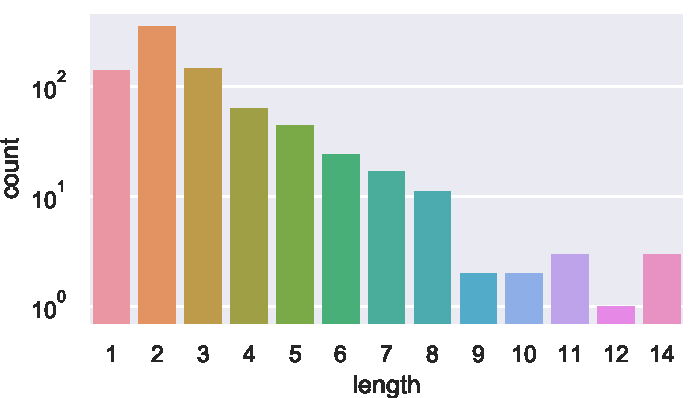
\includegraphics[width=\linewidth]{figs/lengths.pdf}
    \vspace{-10pt}
\end{figure}
Referring expressions vary in length but are mostly short.
\paragraphbreak

\begin{figure}[t]
    \centering
    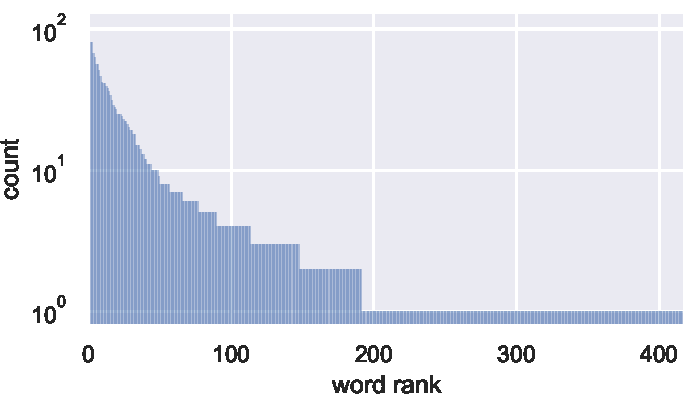
\includegraphics[width=\linewidth]{figs/freqs.pdf}
    \vspace{-10pt}
\end{figure}
Words are Zipfian distributed across the referring expressions.

}
\end{block}

\end{column}	%%% END COLUMN 1 %%%

%%%%%%%%%%%%%%%%%%%%%%%%%%%%%%%%%%%%%%%%%%%%%%%%%%%%%%%%%%%%%%%%%%%%%%%%%%%%%%%%%%%%%%%%%%%
\begin{column}{\centercolumnwidth\linewidth}    %%% COLUMN 2 %%%

\begin{block}{\setblocksize Punchline}
%\vspace{-30pt}
  \vspace{1mm}
\justifying{\Huge
Referring expressions and pictures of individual objects improve robot success detection for object stacking and nesting!
}
\end{block}

\begin{block}{\setblocksize }
%\vspace{-30pt}
  \vspace{1mm}
\justifying{\setcentersize

% \begin{figure}[!t]
%   \centering
%   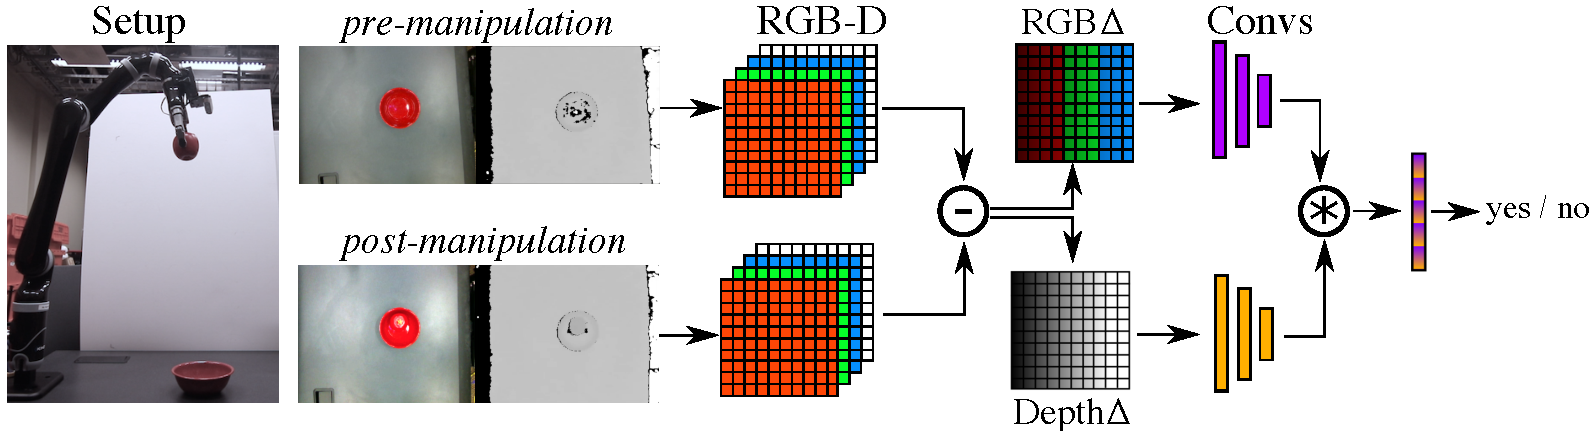
\includegraphics[width=\linewidth]{figs/RGBD.pdf}
% \end{figure}
% The \ego{} architecture is trained to detect whether the grasped object is either \IN{} (nested) or \ON{} (stacked) the target object after manipulation given egocentric scans.

\begin{figure}
  \centering
  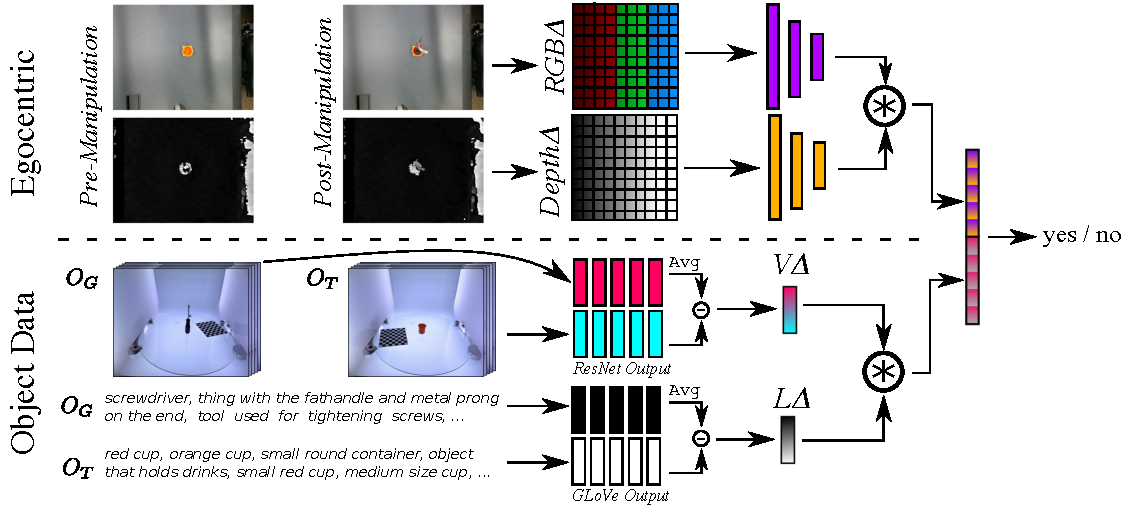
\includegraphics[width=\linewidth]{figs/RGBD+L+V.pdf}    
\end{figure}
The full architecture takes egocentric visual input, vision embeddings from multiple static image viewpoints of each object, and language embeddings from referring expressions for each object.
\paragraphbreak
\paragraphbreak

\begin{table}
    \centering
    \large
    \begin{tabular}{@{}c>{\columncolor[gray]{0.9}}ccp{16em}>{\columncolor[gray]{0.9}}cc}% p{9em}@{}}
    \toprule
    \textbf{Egocentric}
    \hfill $\Rightarrow$ & Pred & 
    \multicolumn{2}{l}\textbf{Egocentric + Pretrained Object} \hfill $\Rightarrow$ & Pred & Truth \\% & Reason\\
    \midrule
    \raisebox{-.8\height}{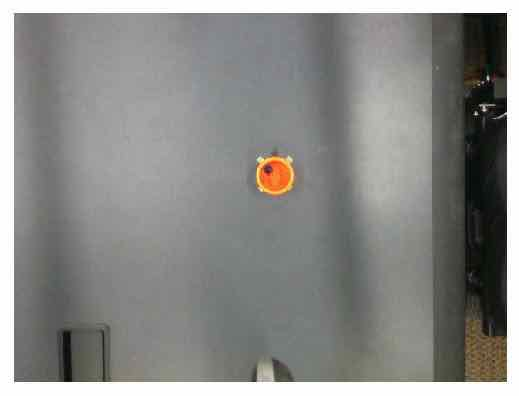
\includegraphics[width=0.15\linewidth]{figs/063-f_marbles+065-a_cups+rgb.jpeg}} 
    & \multirow{2}{*}{\cellcolor{red!25}\xmark In} 
        & \raisebox{-0.8\height}{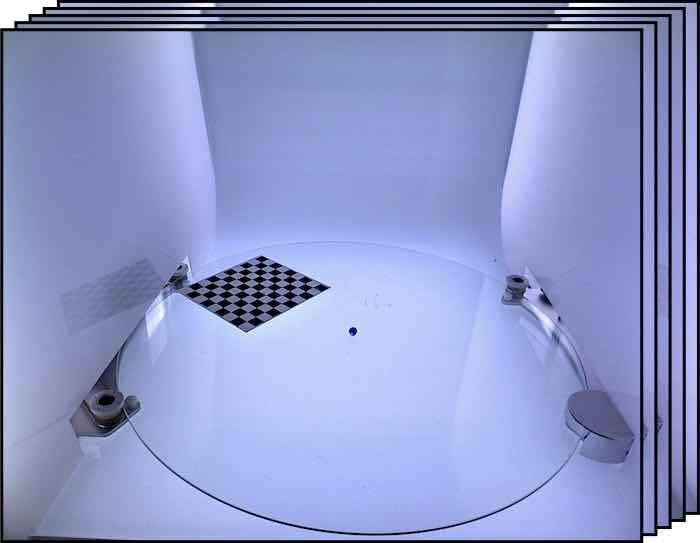
\includegraphics[width=0.14\linewidth]{figs/063-f_marbles-stack.jpeg}} & \textit{small black sphere}, \textit{round black item}, \textit{small marble}, \textit{the blue object}, \textit{round object}, \textit{tiny object}, \textit{tiny dot}, \textit{blue round object}, \textit{little ball} & \multirow{2}{*}{\cellcolor{blue!25} \cmark In} 
        & \multirow{2}{*}{\cmark In} \\%\multirow{2}{9em}{With egocentric vision alone, it is difficult to see the small marble.
        % After adding object data, the model classifies the \textit{tiny} marble \IN{} the \textit{cup} container.} \\
    \raisebox{-.8\height}{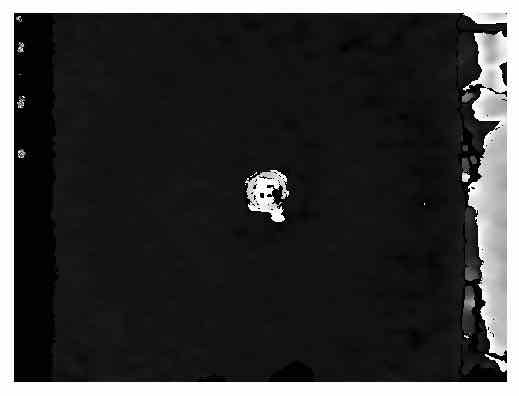
\includegraphics[width=0.15\linewidth]{figs/063-f_marbles+065-a_cups+d.jpeg}}
    & \cellcolor{red!25}
        & \raisebox{-.8\height}{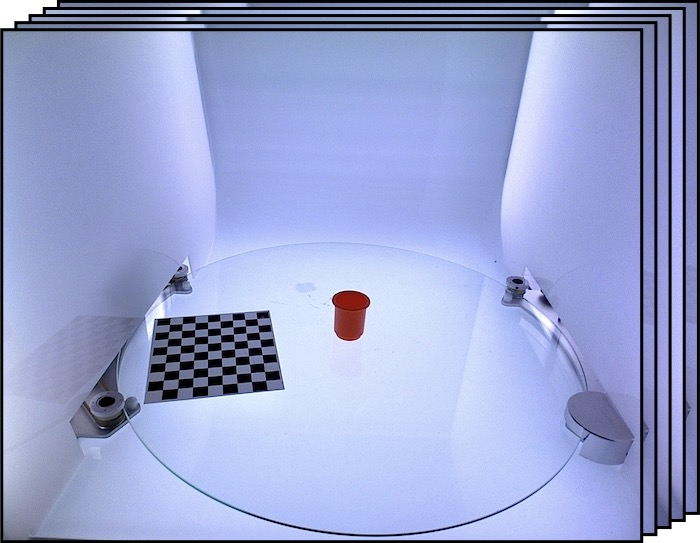
\includegraphics[width=0.14\linewidth]{figs/065-a_cups-stack.jpeg}} & \textit{red cup}, \textit{orange cup}, \textit{small round container}, \textit{object that holds drinks}, \textit{small red cup}, \textit{red cup}, \textit{medium size cup without handles}, \textit{red plastic thing}, \textit{red cylinder} & \cellcolor{blue!25} & \\ %& &  \\
    \midrule
       \raisebox{-.9\height}{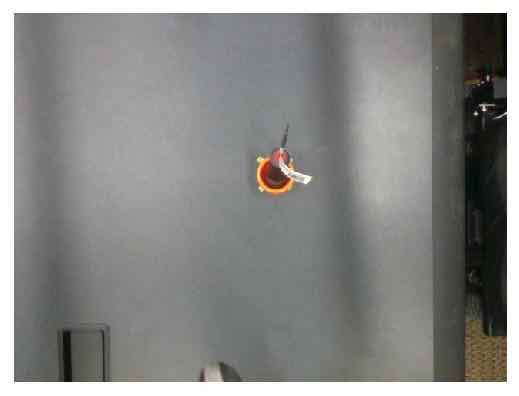
\includegraphics[width=0.15\linewidth]{figs/044_flat_screwdriver+065-a_cups+rgb.jpeg}} 
       & \multirow{2}{*}{\cellcolor{red!25} \xmark In} 
        & \raisebox{-.9\height}{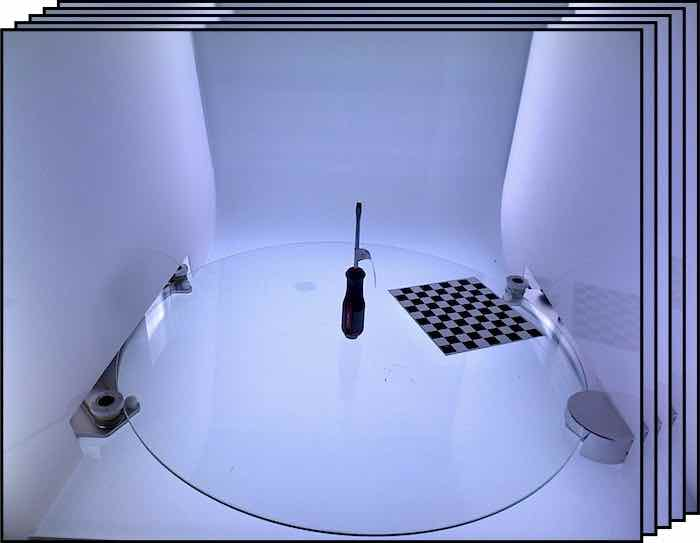
\includegraphics[width=0.14\linewidth]{figs/044_flat_screwdriver-stack.jpeg}} & \textit{screwdriver}, \textit{thing with the fat handle and metal prong on the end}, \textit{tool used for tightening screws}, \textit{screw driver with long tip}, \textit{screwdriver}, \textit{plastic handle screw driver}, \textit{non phillips screw driver}, \textit{tool}, \textit{black screwdriver} & \multirow{2}{*}{\cellcolor{blue!25} \cmark In} 
        & \multirow{2}{*}{\cmark In} \\ % & \multirow{2}{9em}{The reflective screwdriver and its tag spill over the edge of the cup, creating a misleading egocentric depth scan.
        % After adding object data, the model classifies the \textit{screwdriver} as being \IN{} the \textit{cup} container.} \\
    \raisebox{-.8\height}{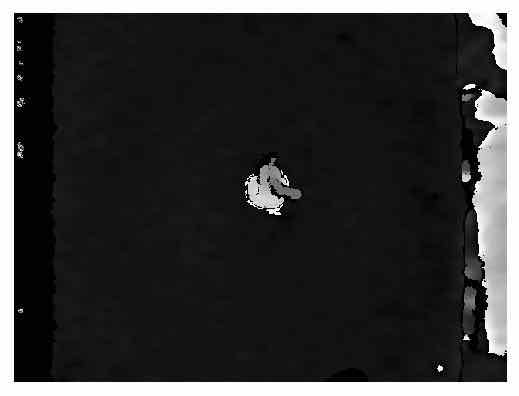
\includegraphics[width=0.15\linewidth]{figs/044_flat_screwdriver+065-a_cups+d.jpeg}} 
    & \cellcolor{red!25}
        & \raisebox{-.8\height}{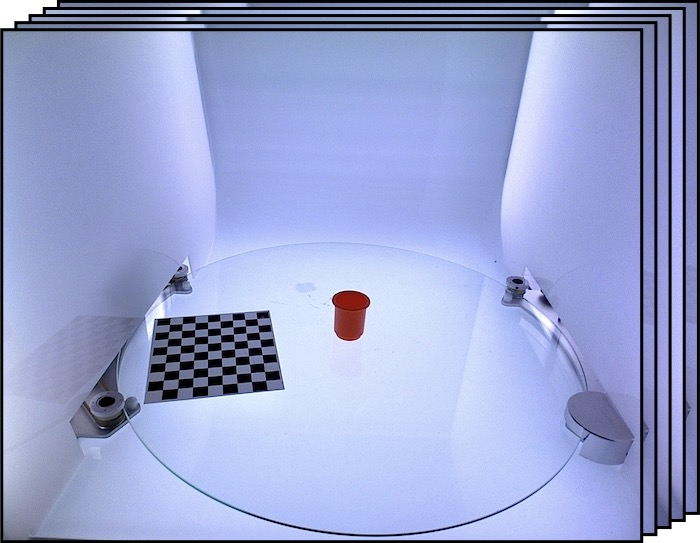
\includegraphics[width=0.14\linewidth]{figs/065-a_cups-stack.jpeg}} & \textit{red cup}, \textit{orange cup}, \textit{small round container}, \textit{object that holds drinks}, \textit{small red cup}, \textit{red cup}, \textit{medium size cup without handles}, \textit{red plastic thing}, \textit{red cylinder} & \cellcolor{blue!25} & \\% &  &  \\
    \midrule
       \raisebox{-.8\height}{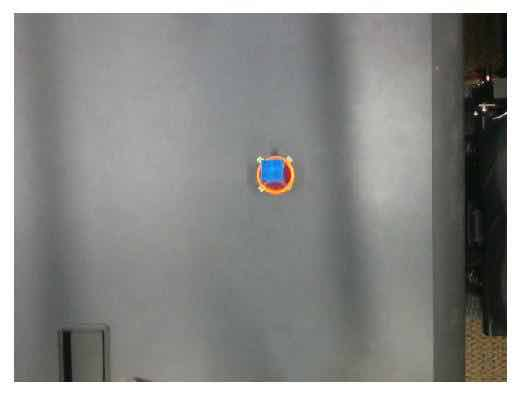
\includegraphics[width=0.15\linewidth]{figs/073-g_lego_duplo+065-a_cups+rgb.jpeg}} 
       & \multirow{2}{*}{\cellcolor{red!25} \xmark On} 
        & \raisebox{-.8\height}{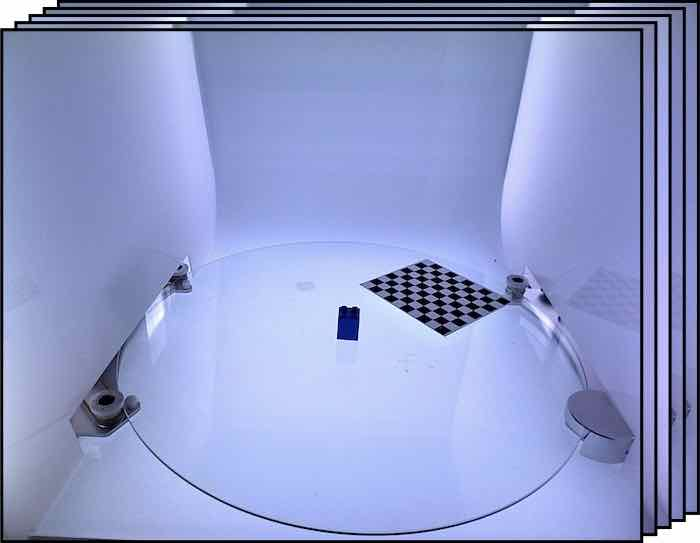
\includegraphics[width=0.14\linewidth]{figs/073-g_lego_duplo-stack.jpeg}} & \textit{blue thing}, \textit{blue plastic rectangle}, \textit{blue plastic block}, \textit{blue cube}, \textit{lego piece}, \textit{blue plastic thing}, \textit{blue block}, \textit{small square block}, \textit{little blue block} & \multirow{2}{*}{\cellcolor{blue!25} \cmark On} 
        & \multirow{2}{*}{\cmark On} \\ % & \multirow{2}{9em}{The block rests partially nested in the cup, exhibiting a rare hybrid of both \ON{} modalities (resting on top versus nested inside).
        % After adding object data, the \textit{small block} is classified as resting \ON{} the \textit{cup} container.} \\
    \raisebox{-.8\height}{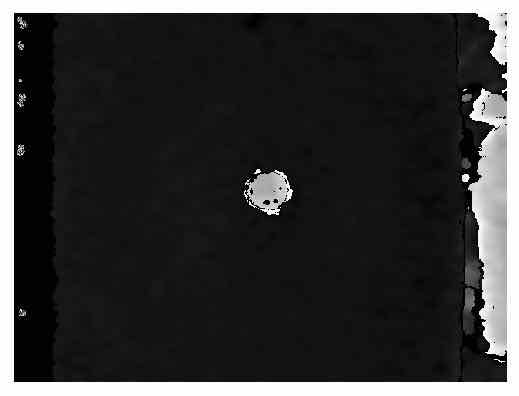
\includegraphics[width=0.15\linewidth]{figs/073-g_lego_duplo+065-a_cups+d.jpeg}} 
    & \cellcolor{red!25}
        & \raisebox{-.8\height}{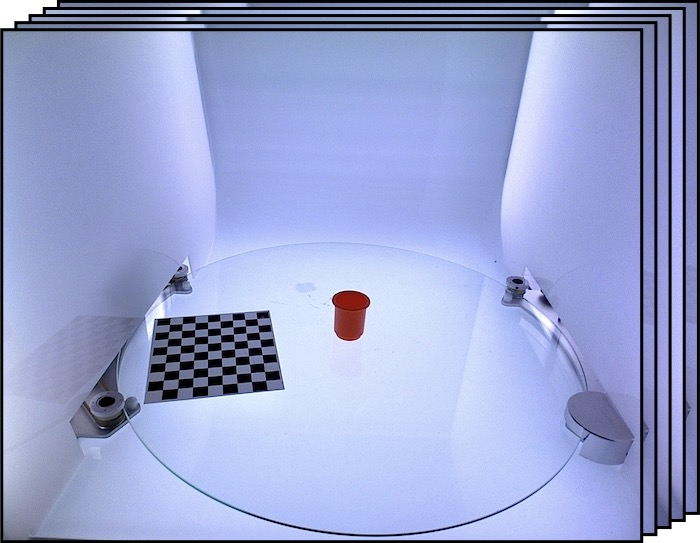
\includegraphics[width=0.14\linewidth]{figs/065-a_cups-stack.jpeg}} & \textit{red cup}, \textit{orange cup}, \textit{small round container}, \textit{object that holds drinks}, \textit{small red cup}, \textit{red cup}, \textit{medium size cup without handles}, \textit{red plastic thing}, \textit{red cylinder} & \cellcolor{blue!25} & \\ % & &  \\
    \midrule
    \raisebox{-.9\height}{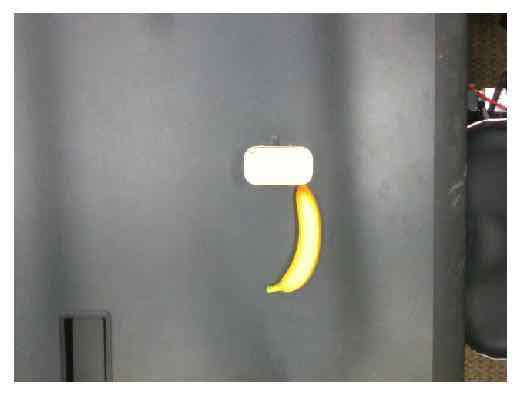
\includegraphics[width=0.15\linewidth]{figs/011_banana+010_potted_meat_can+rgb.jpeg}} 
    & \multirow{2}{*}{ \cellcolor{blue!25} \xmark On} 
        & \raisebox{-0.9\height}{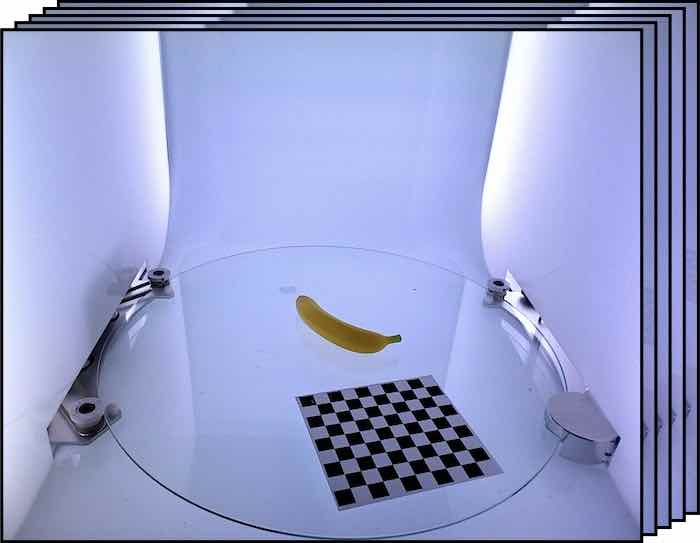
\includegraphics[width=0.14\linewidth]{figs/011_banana-stack.jpeg}} & \textit{yellow thing}, \textit{long yellow item}, \textit{soft yellow thing}, \textit{yellow curved cylinder}, \textit{yellow fruit}, \textit{the object that is mostly yellow with slight green at one of the tips}, \textit{yellow long fruit}, \textit{yellow banana}, \textit{banana} & \multirow{2}{*}{\cellcolor{red!25} \cmark On} 
        & \multirow{2}{*}{\xmark On} \\ % & \multirow{2}{9em}{Given object data predictions pretrained on crowdsourced labels, the model predicts that \textit{fruit} is balanced \ON{} the \textit{can}, consistent with human ability.
        % In reality, the robot manipulator lacks the dexterity to reliably balance the banana.} \\
    \raisebox{-.8\height}{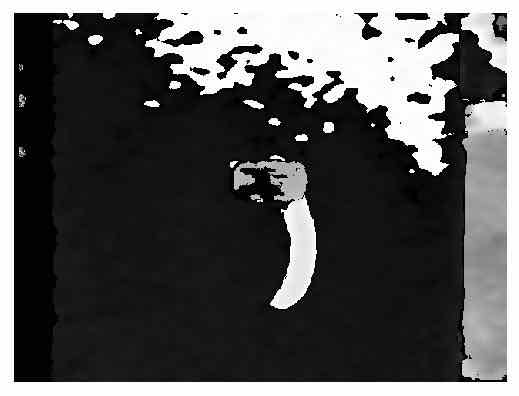
\includegraphics[width=0.15\linewidth]{figs/011_banana+010_potted_meat_can+d.jpeg}}
    & \cellcolor{blue!25}
        & \raisebox{-.8\height}{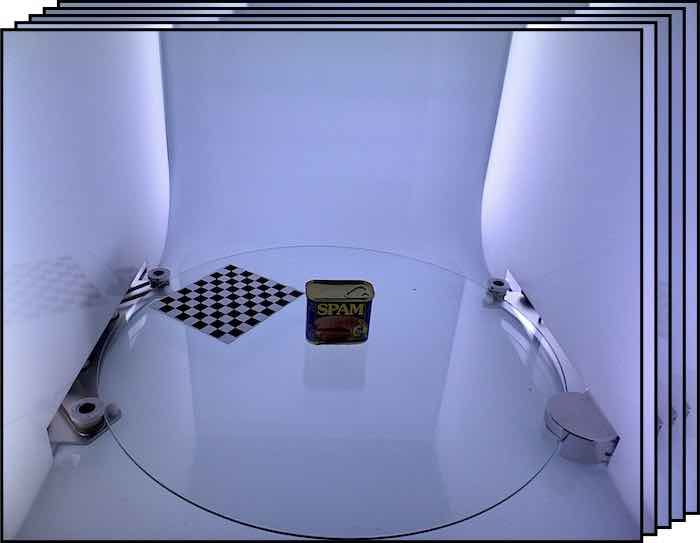
\includegraphics[width=0.14\linewidth]{figs/010_potted_meat_can-stack.jpeg}} & \textit{spam}, \textit{canned meat}, \textit{metal can}, \textit{can of spam}, \textit{aluminum cube}, \textit{blue and gold cube}, \textit{rectangular can}, \textit{square}, \textit{glass circle} & \cellcolor{red!25} & \\ % & &  \\
    \bottomrule
    \end{tabular}
\end{table}

}
\end{block}

\end{column}  %%% END COLUMN 2 %%%

%%%%%%%%%%%%%%%%%%%%%%%%%%%%%%%%%%%%%%%%%%%%%%%%%%%%%%%%%%%%%%%%%%%%%%%%%%%%%%%%%%%%%%%%%%%
\begin{column}{\sidecolumnwidth\linewidth}    %%% COLUMN 3 %%%

\begin{block}{\setblocksize Evaluation and Ablations}
%\vspace{-30pt}
	\vspace{1mm}
\justifying{\setsize

The dataset consists of pairs of YCB objects $Y$ and containers $C$, split into folds.
For a subset of pairs, we have egocentric, \textbf{Robot} manipulation data.
\begin{table}
\begin{center}
\centering
\begin{tabular}{l r r | r r | r r}
    \toprule
    & \multicolumn{2}{c}\textbf{Objects} & \multicolumn{2}{c}\textbf{Robot} & \multicolumn{2}{c}\textbf{All\phantom{00}} \\
  \textbf{Fold} & $Y$ & $C$ & \IN{} & \ON{} & \IN{} & \ON{} \\
  \midrule
  Train & $51$ & $17$ & $191$ & $191$ & $800$ & $2500$ \\
  Dev & $20$ & $5$ & $47$ & $58$ & $100$ & $400$ \\
  Test & $19$ & $6$ & $60$ & $60$ & $114$ & $361$ \\
  \bottomrule
\end{tabular}
\end{center}
\end{table}
\paragraphbreak
\paragraphbreak

\checkmark indicates signal was included, while ``pre" indicates models with object features pretrained from \textbf{All Pairs} of available objects.

\begin{table}[t]
\centering \large
\begin{tabular}{l c c c r r}
  \toprule
    & \multicolumn{3}{c}\textbf{Model ($M$)} & \multicolumn{2}{c}\textbf{Detection Correct $\uparrow$} \\
  & \multirow{2}{*}{Ego} & \multicolumn{2}{c}{Object Data} & \\
  & & Lang & Vis & \multicolumn{1}{c}{\IN{}} & \multicolumn{1}{c}{\ON{}} \\
  \midrule
  \multirow{14}{*}{\rotatebox{90}{\textit{Dev Fold}}}
  % & & & & & \\
  & \zv & \checkmark & \zv & $.70\pm.03$ & $.56\pm.10$ \\
  & \zv & pre & \zv & $.72\pm.04$ & $.57\pm.09$ \\
  & \zv & \zv & \checkmark & $.71\pm.08$ & $.50\pm.06$ \\
  & \zv & \zv & pre & $.72\pm.07$ & $.53\pm.05$ \\
  & \zv & \checkmark & \checkmark & $.76\pm.08$ & $.58\pm.05$ \\
  & \zv & pre & pre & $\pmb{.78}\pm.08$ & $.60\pm.04$ \\
  \cmidrule{2-6}
  % & \checkmark & \zv & \zv & $.65\pm.03$ & $.56\pm.11$ \\
  & \checkmark & \checkmark & \zv & $.67\pm.08$ & $.60\pm.08$ \\
  & \checkmark & pre & \zv & $.68\pm.08$ & $\pmb{.62}\pm.08$ \\
  & \checkmark & \zv & \checkmark & $.70\pm.10$ & $.58\pm.11$ \\
  & \checkmark & \zv & pre & $.72\pm.08$ & $.59\pm.13$ \\
  & \checkmark & \checkmark & \checkmark & $.70\pm.09$ & $.59\pm.07$ \\
  & \checkmark & pre & pre & $.73\pm.09$ & $.62\pm.07$ \\
  \cmidrule{2-6}
  & \multicolumn{3}{l}{Baseline (MC)} & $.32\pm.00$ & $.36\pm.00$ \\
  & \multicolumn{3}{l}{Baseline (Rand)} & $.49\pm.06$ & $.50\pm.06$ \\
  \midrule
  \multirow{14}{*}{\rotatebox{90}{\textit{Test Fold}}} 
  % & & & & & \\
  & \zv & \checkmark & \zv & $.79\pm.02$ & $.45\pm.05$ \\
  & \zv & pre & \zv & $.79\pm.02$ & $.48\pm.07$ \\
  & \zv & \zv & \checkmark & $\pmb{.80}\pm.04$ & $.46\pm.09$ \\
  & \zv & \zv & pre & $.81\pm.04$ & $.48\pm.06$ \\
  & \zv & \checkmark & \checkmark & $\pmb{.80}\pm.03$ & $.55\pm.04$ \\
  & \zv & pre & pre & $.79\pm.04$ & $.55\pm.04$ \\
  \cmidrule{2-6}
  % & \checkmark & \zv & \zv & $.76\pm.06$ & $.54\pm.12$ \\
  & \checkmark & \checkmark & \zv & $.75\pm.06$ & $.54\pm.10$ \\
  & \checkmark & pre & \zv & $\pmb{.80}\pm.02$ & $.57\pm.07$ \\
  & \checkmark & \zv & \checkmark & $.75\pm.11$ & $.57\pm.10$ \\
  & \checkmark & \zv & pre & $\pmb{.80}\pm.05$ & $.56\pm.10$ \\
  & \checkmark & \checkmark & \checkmark & $.74\pm.07$ & $\pmb{.59}\pm.08$ \\
  & \checkmark & pre & pre & $.77\pm.05$ & $\pmb{.59}\pm.06$ \\
  \cmidrule{2-6}
    & \multicolumn{3}{l}{Baseline (MC)} & $.20\pm.00$ & $.32\pm.00$ \\
    & \multicolumn{3}{l}{Baseline (Rand)} & $.52\pm.05$ & $.51\pm.07$ \\
  \bottomrule
\end{tabular}
\end{table}
Performance on \textbf{Robot Pairs}.
\paragraphbreak
\paragraphbreak

\begin{table}[t]
\centering \large
\begin{tabular}{l c c r r}
  \toprule
    & \multicolumn{2}{c}\textbf{Model ($M$)} & \multicolumn{2}{c}\textbf{Prediction Correct $\uparrow$} \\
  & \multicolumn{2}{c}{Object Data} & & \\
  & Lang & Vis & \multicolumn{1}{c}{\IN{}} & \multicolumn{1}{c}{\ON{}} \\
  \midrule
  \multirow{5}{*}{\rotatebox{90}{\emph{Dev Fold}}}
  % & & & $.87\pm.00$ & $.73\pm.00$ \\
  & \checkmark & \zv & $.86\pm.02$ & $.76\pm.01$ \\
  & \zv & \checkmark & $.94\pm.01$ & $.79\pm.01$ \\
  & \checkmark & \checkmark & $.86\pm.04$ & $.78\pm.01$ \\
  \cmidrule{2-5}
  & \multicolumn{2}{l}{Baseline (MC)} & $.87\pm.00$ & $.73\pm.00$ \\
  & \multicolumn{2}{l}{Baseline (Rand)} & $.49\pm.07$ & $.50\pm.03$ \\
  \midrule
  \multirow{5}{*}{\rotatebox{90}{\emph{Test Fold}}} 
  % & & & $.84\pm.00$ & $.83\pm.00$ \\
  & \checkmark & \zv & $.86\pm.01$ & $.83\pm.01$ \\
  & \zv & \checkmark & $.88\pm.02$ & $.82\pm.01$ \\
  & \checkmark & \checkmark & $.87\pm.02$ & $.83\pm.01$ \\
  \cmidrule{2-5}
    & \multicolumn{2}{l}{Baseline (MC)} & $.84\pm.00$ & $.83\pm.00$ \\
    & \multicolumn{2}{l}{Baseline (Rand)} & $.51\pm.06$ & $.51\pm.03$ \\
  \bottomrule
\end{tabular}
\end{table}
Performance on \textbf{All Pairs}.

}
\end{block}

\end{column}	%%% END COLUMN 3 %%%

%%%%%%%%%%%%%%%%%%%%%%%%%%%%%%%%%%%%%%%%%%%%%%%%%%%%%%%%%%%%%%%%%%%%%%%%%%%%%%%%%%%%%%%%%%%%%%%%%%%%
\end{columns}

\end{frame}

\end{document}


%%%%%%%%%%%%%%%%%%%%%%%%%%%%%%%%%%%%%%%%%%%%%%%%%%%%%%%%%%%%%%%%%%%%%%%%%%%%%%%%%%%%%%%%%%%%%%%%%%%%
%%% Local Variables: 
%%% mode: latex
%%% TeX-PDF-mode: t

